%! Author = domore
%! Date = 8/11/21

% Preamble
\documentclass[11pt]{article}

% Packages
\usepackage{amsmath}
\usepackage{graphicx}
\usepackage{hyperref}
\hypersetup{
    colorlinks=true,
    linkcolor=blue,
    filecolor=magenta,
    urlcolor=cyan,
    citecolor=blue
}
\usepackage{cleveref}
\usepackage[margin=1.1in]{geometry}
\usepackage{python}
\usepackage{pythontex}
% Documentation
% https://raw.githubusercontent.com/gpoore/pythontex/master/pythontex/pythontex.pdf
% tricks
% https://raw.githubusercontent.com/gpoore/pythontex/master/pythontex_gallery/pythontex_gallery.tex
% compilation
%pdflatex -aux-directory=/home/domore/PycharmProjects/ds_project-1/document_files/aux -output-directory=/home/domore/PycharmProjects/ds_project-1 main_document.tex
%python document_files/pythontex/pythontex3.py document_files/main_document.tex
%pdflatex -aux-directory=/home/domore/PycharmProjects/ds_project-1/document_files/aux -output-directory=/home/domore/PycharmProjects/ds_project-1 main_document.tex
\usepackage[framemethod=TikZ]{mdframed}
\usepackage{booktabs}
%\usepackage{multirow}
\usepackage{rotating}

% for future projects
% \usepackage[usefamily=juliacon]{pythontex}

% Document
\begin{document}

\part[wine]{Project 1: Wine quality} \label{part:wine}

\section*{Introduction}
In the paragraphs to come we will discuss different approaches and models to be used in the dataset used in~\cite{wine}.

The following dataset consist of different a sample of wines with different characteristics and their relevant
quality.
The box below has an overview description of the dataset we will analyse.
A further description of each variable can be found in \Cref{tab:description_wine}.

% these lines will not be presented in the pdf
% pyconcode only excecutes (does not show code)
%! suppress = EscapeUnderscore
%! suppress = EscapeHashOutsideCommand
\begin{pyconcode}
import pandas as pd
import os

# Referencing folders and data names
path = os.getcwd()
# We have to re-structure the path since we are in LaTeX
path = os.path.abspath(os.path.join(path, os.pardir))
file_name = 'winequality-red.csv'
path_file = f'{path}/code_python/project1_wine/data/{file_name}'
# We load the data and present an overview
wine_data = pd.read_csv(path_file)
\end{pyconcode}

%! suppress = EscapeUnderscore
\begin{pyconsole}[][frame=single]
wine_data.info()
wine_data.describe().round(decimals=2).transpose()
\end{pyconsole}

\section*{Exploratory analysis}

To avoid unnecessary analysis, first we will perform a few checks to get a deeper understanding of the
data we are using.
To that end, we first check that the correlation structure amongst the variables (see \cref{fig:wine_heatmap}),
including the quality of the wine.
This should give us a general idea of how and if the variables are related to one another.


\begin{figure}[h!]
    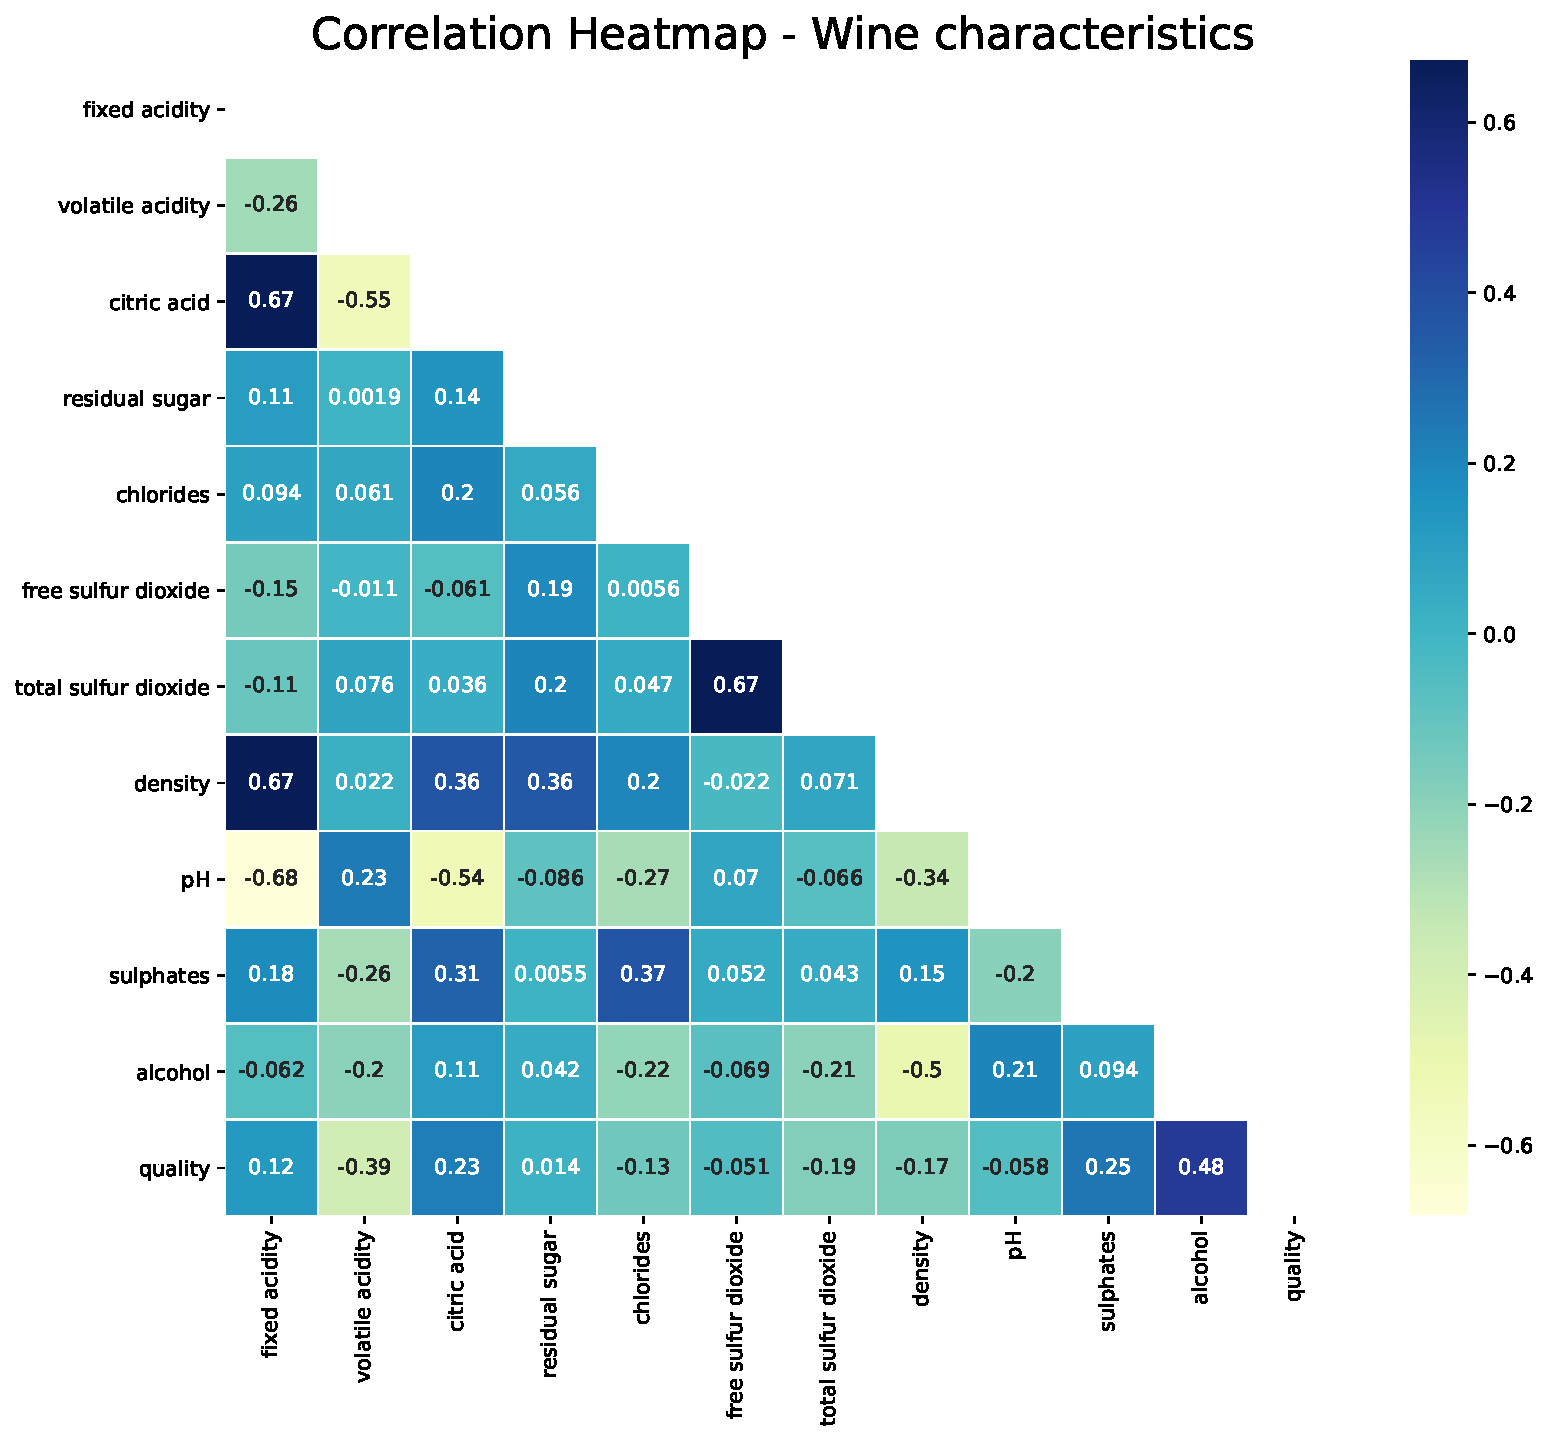
\includegraphics[width=0.9\textwidth]{figs/wine_heatmap}
    \caption{Correlation structure of wine characteristics.}
    \label{fig:wine_heatmap}
\end{figure}


There are a few things we could check whether the data in the data to assess whether what we are looking relates somehow
to our prior knowledge about the topic.
This prior knowledge might help us identify certain links, that might not be obvious if the data were not labeled.

At first glance, one can note that \emph{fixed acidity} and \emph{citric acidity} are strongly correlated (negatively) to the \emph{pH},
although their correlation is not \emph{-1}.
This should relate to our prior knowledge, given that \emph{pH} is directly related to the acidity of a
solution.
Additionally, we can see that \emph{alcohol} correlates negatively with the \emph{density} of the wine.
This makes sense, given that the wine is a solution of different solutes, those in all likelihood are ``heavier''
than the alcohol solute.
Hence, the more the alcohol content increases in the wine, the less dense it becomes.
Another interesting characteristic of the wine that is highly correlated to its quality is the
alcohol content.

\vspace{2pt}
Another visual analysis we could perform is to look at the KDEs (Kernel Density Estimates).
These we could imagine as a cross-sectional cut in a bi-variate probability distribution.
\Cref{fig:wine_kdes} shows us that even though the wines in the sample range from quality 3 to 8
(see subplot in row 3, column 4), it would seem that there are mostly 4 important groups.
The earlier stated fact, ad priori, gives us an interesting thing we should have in mind when trying
to fit any kind of model.
I.e., the tails of the quality (grades 3 and 8) will be underrepresented, then most model we could think
of fitting will have trouble predicting a grade close to 3 and 8 and beyond (to each direction).

\begin{figure}[h!]
    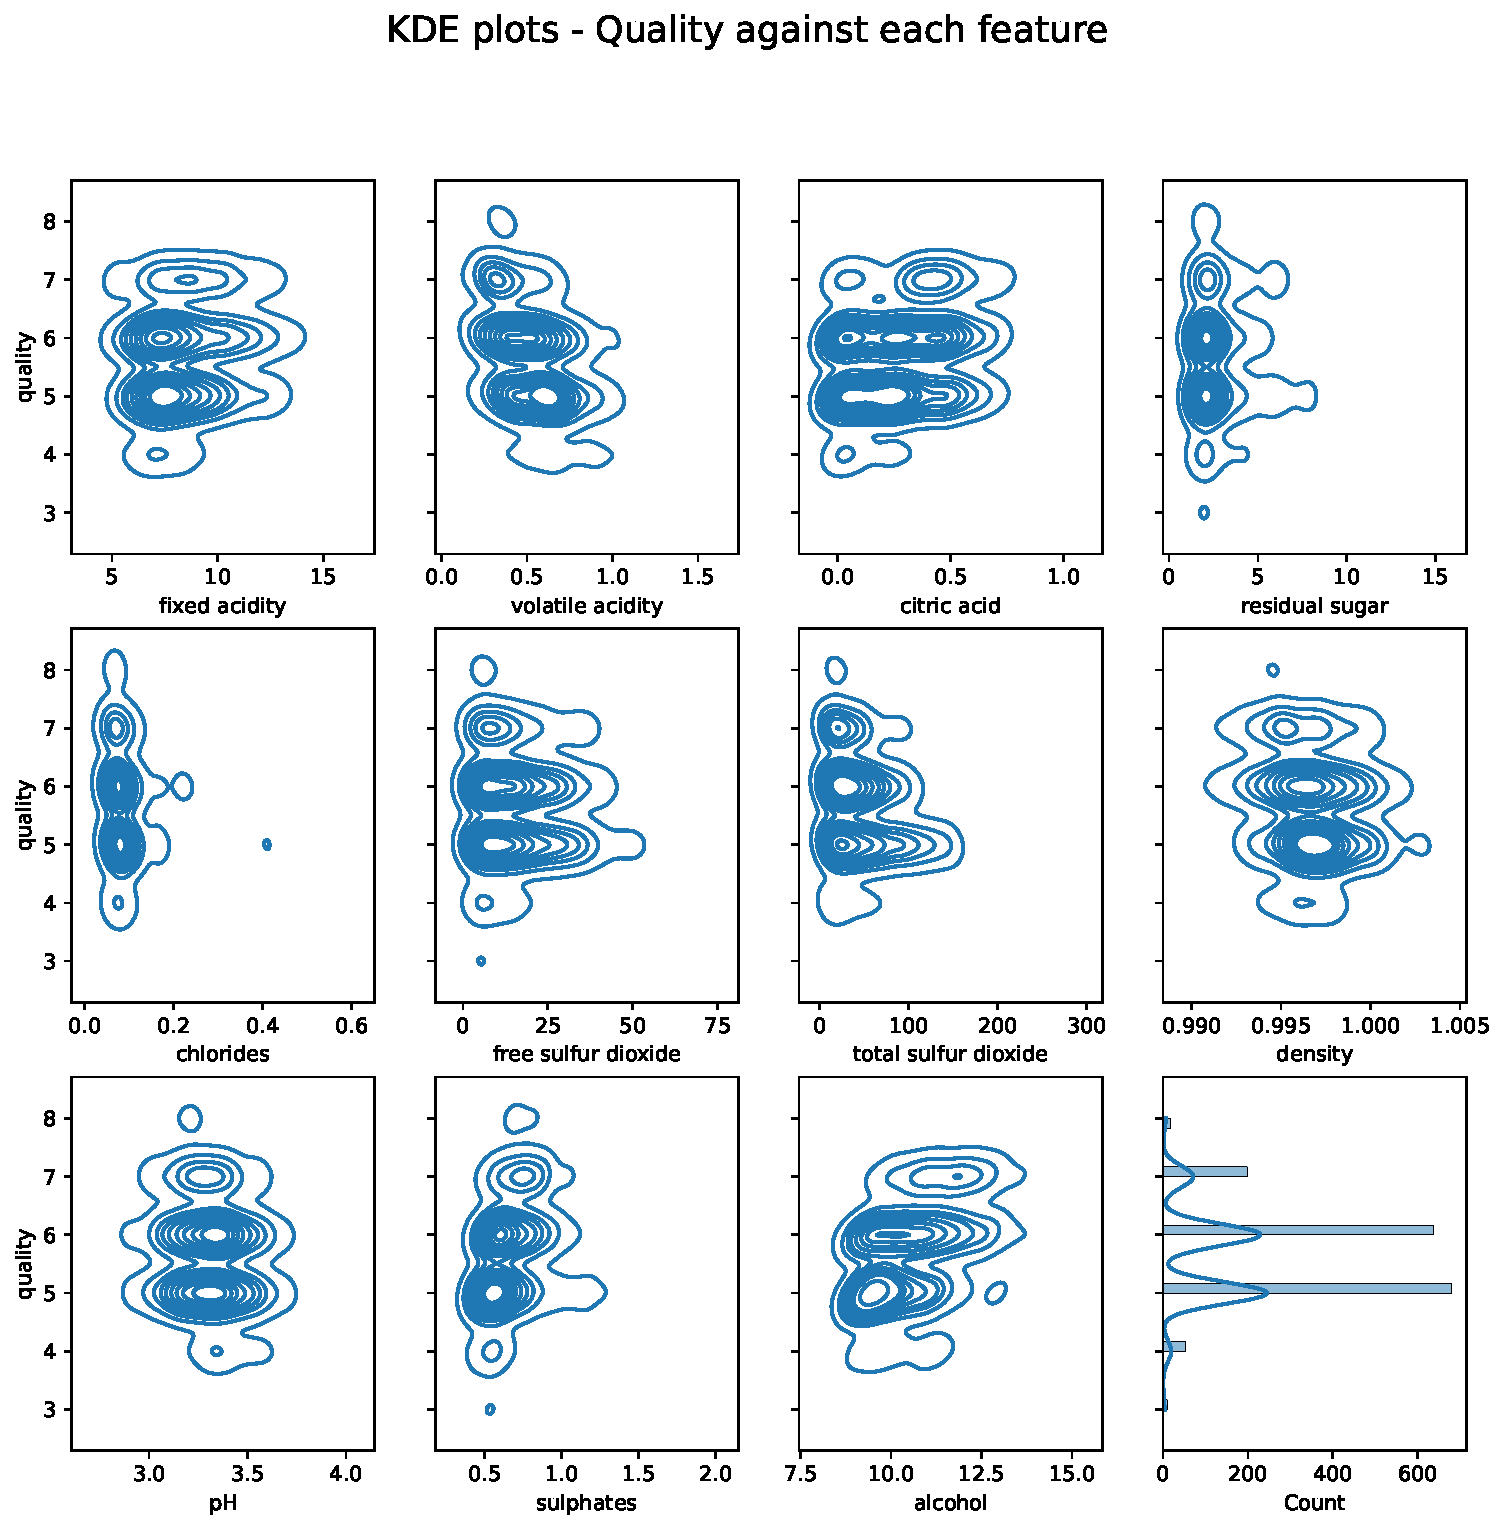
\includegraphics[width=0.9\textwidth]{figs/wine_kde}
    \caption{KDEs for wine features.}
    \label{fig:wine_kdes}
\end{figure}


\section*{Conclusion}

{\color{red}\textbf{[1]}} All these characteristics are important in a wine.
We used all these statistical models to try to understand to which degree they are important
to determine a wine`s quality.
These analyses might be really important for a winemaker to know.
Given that by affecting the inherent characteristics of the wine will most likely have an
impact on the quality of that wine.

\newpage
\part[food]{Project 2: Food Preferences} \label{part:food}


\newpage
\part[stores]{Project 3: Store Sales} \label{part:sales}



\begin{thebibliography}{1}
\bibitem{wine} P. Cortez, A. Cerdeira, F. Almeida, T. Matos and J. Reis. {\em Modeling wine preferences by data mining from physicochemical properties.
In Decision Support Systems, Elsevier, 47(4):547-553},  2009.
\end{thebibliography}




\begin{sidewaystable}
    \centering
    \caption{Description of wine characteristics.}
    \resizebox{\columnwidth}{!}{
    \begin{tabular}{ll}
\toprule
      Characteristic &                                                                                                                                                                                      Description \\
\midrule
       fixed acidity &                                                                                                                most acids involved with wine or fixed or nonvolatile (do not evaporate readily). \\
    volatile acidity &                                                                                         the amount of acetic acid in wine, which at too high of levels can lead to an unpleasant, vinegar taste. \\
      citric acidity &                                                                                                                  found in small quantities, citric acid can add "freshness" and flavor to wines. \\
      residual sugar &                     the amount of sugar remaining after fermentation stops, it`s rare to find wines with less than 1 gram/liter and wines with greater than 45 grams/liter are considered sweet. \\
           chlorides &                                                                                                                                                                  the amount of salt in the wine. \\
 free sulfur dioxide &                                the free form of SO2 exists in equilibrium between molecular SO2 (as a dissolved gas) and bi-sulfate ion; it prevents microbial growth and the oxidation of wine. \\
total sulfur dioxide & amount of free and bound forms of S02; in low concentrations, SO2 is mostly undetectable in wine, but at free SO2 concentrations over 50 ppm, SO2 becomes evident in the nose and taste of wine. \\
             density &                                                                                               the density of water is close to that of water depending on the percent alcohol and sugar content. \\
                  pH &                                                          describes how acidic or basic a wine is on a scale from 0 (very acidic) to 14 (very basic); most wines are between 3-4 on the pH scale. \\
           sulphates &                                                                         a wine additive which can contribute to sulfur dioxide gas (S02) levels, which acts as an antimicrobial and antioxidant. \\
             alcohol &                                                                                                                                                         the percent alcohol content of the wine. \\
             quality &                                                                                                                                 output variable (based on sensory data, score between 0 and 10). \\
\bottomrule
\end{tabular}


    }
    \label{tab:description_wine}
\end{sidewaystable}





\end{document}